\section{HACCP e Nutrizione}

L'HACCP ha rivoluzionato l'approccio igienico nei confronti degli
alimenti. Cosa si intende per igiene degli alimenti? L'igiene tutela la
salute; allora l'igiene degli alimenti viene definito nel regolamento
del 2004 come ``l'insieme di tutte quelle misure necessarie a garantire
la sicurezza di un alimento, quindi controllarne i pericoli e che sia
idoneo al consumo, cioè che non rechi danno''.

\subsection{Alimenti come veicolo di infezione}

Ricordiamo che gli alimenti possono essere un veicolo di infezione.
Esistono due categorie di patologie legate agli alimenti, ciascuna con
caratteristiche peculiari:

\begin{itemize}
\item
  \textbf{Malattie infettive a trasmissione fecale-orale} in cui gli
  \emph{alimenti sono dei veicoli efficienti ma non indispensabili},
  infatti sono malattie che possono essere trasmesse anche in altro
  modo. Se io ho una contaminazione da materiale fecale-orale, tocco
  questa superficie e mi porto le mani alla bocca la trasmissione
  avviene lo stesso. Quindi nelle malattie a trasmissione fecale-orale
  l'alimento costituisce un veicolo importante.

In genere hanno un lungo periodo d'incubazione (per es. epatite A,
Poliomielite, Colera)

\item
  \textbf{Tossinfezioni alimentari} (per es. tossinfezione da
  stafilococco, botulismo). \emph{L'alimento è indispensabile perché in
  esso il microrganismo si moltiplica}; sono necessarie alte cariche
  microbiche e sono trasmesse solo da alimenti. Il periodo di
  incubazione è breve, anche di 2 ore per esempio.
\end{itemize}

L'igiene alimentare quindi mira a controllare il pericolo. Che cos'è il
pericolo? E la differenza con il rischio?

\textbf{Il pericolo} è un agente, una condizione; il microrganismo è il
pericolo, oppure una sostanza chimica che ha la potenzialità di causare
danno.

\textbf{Il rischio} è la probabilità che il danno si verifichi. Può
essere presente il pericolo, ma affinché ci sia danno servono
l'esposizione e la vulnerabilità del soggetto (e anche una certa carica
microbica).

\subsection{Tipi di contaminazione}

La contaminazione degli alimenti può avvenire in diversi momenti del
processo che va dalla produzione al consumo.

\begin{itemize}
\item
  \textbf{Contaminazione primaria}: presente nell'alimento all'origine;
  è la materia prima ad essere contaminata (esempi: microrganismi nelle
  cozze, salmonelle nelle uova, contaminanti nella carne di pollo, nella
  frutta e nella verdura\ldots{}).
\item
  \textbf{Contaminazione secondaria}: si verifica durante il processo di
  lavorazione dell'alimento (per esempio quando le persone contaminano
  con Staphylococcus aureus le superfici durante le lavorazioni).
\item
  \textbf{Contaminazione terziaria}: avviene durante la conservazione
  del prodotto.
\item
  \textbf{Contaminazione quaternaria}: avviene durante la distribuzione,
  al momento del consumo (per esempio nelle mense).
\end{itemize}

Quindi è necessario l'igiene nelle materie prime, ma anche in tutto il
processo di lavorazione e distribuzione.

Ci sono fattori che influenzano crescita e sopravvivenza dei
microrganismi; un alimento può essere contaminato, ma se il
microrganismo non trova le condizioni ideali non si sviluppa. Questi
sono elementi sfruttati nella conservazione degli alimenti:

\begin{itemize}
\item
  \textbf{Temperatura}: i microrganismi patogeni si sono ben adattati
  alle temperature del corpo umano (microrganismi mesofili), ma alcuni
  sopravvivono anche in frigorifero (per esempio le muffe)
\item
  \textbf{Ph}: è altresì importante; i microrganismi hanno infatti un ph
  ottimale di crescita (in genere tra 6 e 7.5) e sopravvivono poco a
  valori molto bassi (eccezion fatta per muffe e lieviti che tollerano
  ph anche molto acidi)
\item
  \textbf{Acqua libera}: è necessaria al microrganismo per crescere e
  svilupparsi (il parametro va da 0 a 1). Se diminuisco la presenza di
  acqua viene compromessa la sopravvivenza e la moltiplicazione del
  microrganismo (per questo le procedure come la liofilizzazione o
  l'essicazione sono metodi di conservazione molto efficaci)
\item
  \textbf{Ossigeno}: presenza o assenza. Molti microrganismi richiedono
  ossigeno per sopravvivere (e ciò spiega l'efficacia della
  conservazione sottovuoto per esempio), ma esistono anche microrganismi
  anaerobi , per esempio Clostridium botulinum, che in assenza di
  ossigeno trova il suo habitat ideale.
\end{itemize}

\subsection{Storia HACCP}

La contaminazione, ovvero la presenza di un pericolo nell'alimento, è
associata ad un possibile danno per la salute, con problemi economici e
sanitari (per es. epidemie).

Allora si è reso necessario intervenire con \textbf{l'HACCP (Analisi del
pericolo dei punti critici di controllo)} che ha rivoluzionato il
processo di controllo degli alimenti.

Questo sistema di controllo degli alimenti è stato messo a punto alla
NASA perché sappiamo che gli astronauti hanno una compromissione del
sistema immunitario, pertanto si rende necessaria un'alimentazione a
bassa carica microbica.

\emph{Quindi l'approccio di controllare sempre l'alimento finito con
prelievi di campioni da parte dell'autorità sanitaria (che comporta il
buttare molti alimenti) è stato sostituito da un approccio che predilige
il controllo dell'intero processo, affiancato al controllo del prodotto
finito, individuando quali sono i punti in cui ci può essere
contaminazione tramite una collaborazione tra autorità sanitaria e
responsabile dell'industria alimentare.}

La proposta è stata presentata nel 1971 alla ``Conferenza per la
protezione degli alimenti'', entrata poi in Europa con la direttiva
43/93 del 1993. (NB: le direttive dell'Unione Europea necessitano di
tempo per essere recepite dagli stati membri, a differenza dei
regolamenti che divengono immediatamente operativi). L'Italia ha
impiegato 4 anni per recepire tale direttiva, ufficializzandola nel 1997
con il Decreto Legislativo n\textsuperscript{o}155, che ha introdotto l' HACCP.

Cosa viene espresso in questo decreto? Innanzitutto si definisce
``\emph{industria alimentare''} chiunque manipoli alimenti durante un
momento qualsiasi del processo che parte dalla materia prima e arriva
fino al consumo (quindi non solo le industrie, ma anche i bar, i
venditori ambulanti ecc\ldots{}). In queste deve essere individuato un
responsabile che garantisca che tutto ciò che viene svolto in
quell'industria venga effettuato in modo igienico (che non danneggi la
salute), individuando nella propria attività ogni fase in cui ci
potrebbe essere contaminazione. Il sistema HACCP introduce il termine
autocontrollo, trasferendo quindi la responsabilità della sicurezza
degli alimenti dal controllore ufficiale (storicamente la AUSL) al
responsabile di ogni singola industria. Nel manuale dell'autocontrollo
si possono trovare tutte le regole da applicare in queste fasi.

Qui sotto è mostrato un esempio di diagramma di flusso in uso in una
mensa-ristorante.

\begin{figure}[!ht]
\centering
	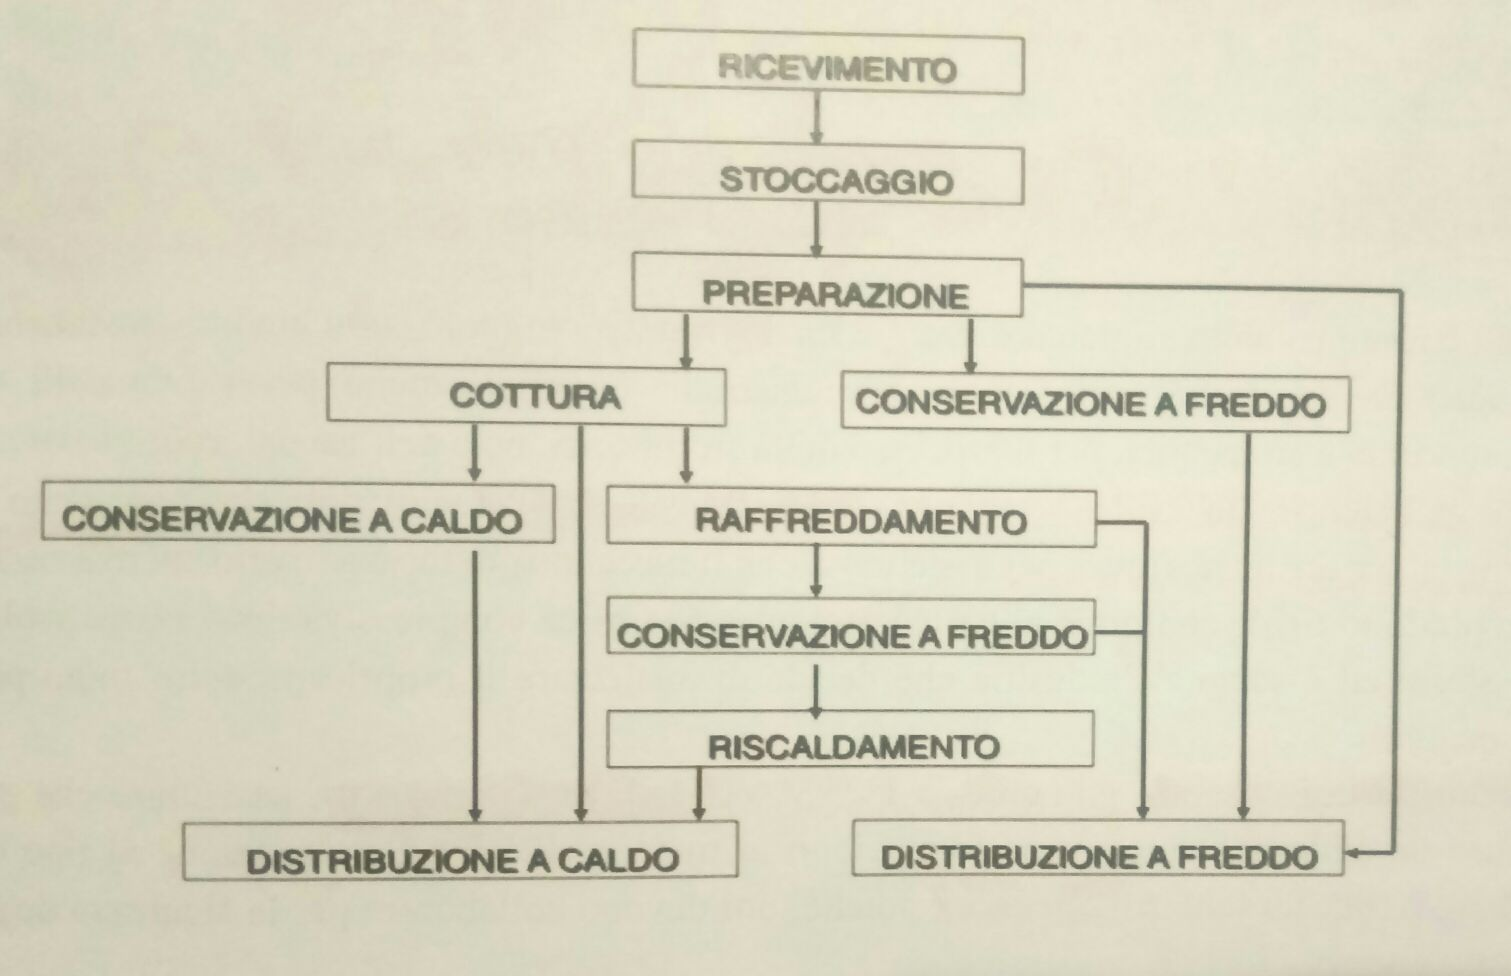
\includegraphics[width=0.7\textwidth]{20/image2.jpeg}
	\end{figure}

Quindi il responsabile deve individuare i punti critici nel diagramma di
flusso a livello dei quali possono essere messi in atto interventi
correttivi per evitare il danno (ad esempio nella conservazione a
freddo, nel caso in cui non tutto l'alimento raggiunga la temperatura
adeguata).

Deve quindi descrivere tutta la sua attività e garantire che siano
mantenute e attuate tutte le procedure avvalendosi dei principi su cui è
basato l'HACCP.

\subsection{Principi HACCP}

Il responsabile deve essere consapevole del suo ruolo e:

\begin{itemize}
\item
  IDENTIFICARE I PERICOLI, ovvero quali microrganismi o sostanze
  potrebbero contaminare quello specifico alimento, e valutare i RISCHI.
\item
  IDENTIFICARE I PUNTI CRITICI DI CONTROLLO, definiti come momenti in
  cui può avvenire la contaminazione ed in cui si può applicare un
  intervento di prevenzione per evitare il danno (per esempio cottura e
  refrigerazione che possono evitare la contaminazione)
\item
  STABILIRE I LIMITI CRITICI, valori che devono essere rispettati
  affinché ogni punto critico sia sotto controllo.
\item
  STABILIRE LE PROCEDURE DI MONITORAGGIO: deve essere tutto scritto nel
  manuale di autocontrollo. Pianificare quindi i controlli, la modalità,
  la periodicità e tutte le procedure conseguenti.
\item
  INDIVIDUARE LE AZIONI CORRETTIVE qualora i limiti non vengano
  rispettati (per esempio buttare l'alimento).
\item
  STABILIRE PROCEDURE DI VERIFICA DI TUTTO IL SISTEMA per accertarsi che
  tutto quello che è stato stabilito funzioni (per esempio il controllo
  dell' alimento finito). La verifica viene fatta ovviamente a
  periodicità predefinite.
\item
  STABILIRE PROCEDURE DI DOCUMENTAZIONE E REGISTRAZIONE: scrivere tutto
  quello che si fa, fare tutto quello che si scrive, monitorare tutto
  quello che si fa e documentare tutto ciò che si fa.
\end{itemize}

Il responsabile dell'industria deve inoltre garantire la FORMAZIONE
degli operatori, poiché tutti devono collaborare per la sicurezza degli
alimenti.

\begin{figure}[!ht]
\centering
	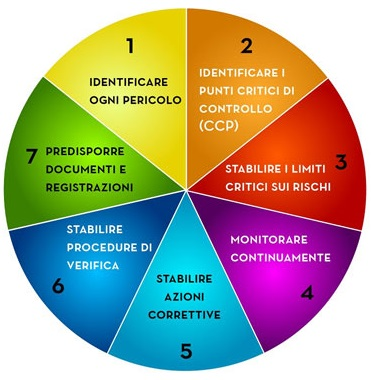
\includegraphics[width=0.7\textwidth]{20/image3.jpeg}
	\end{figure}

L'HACCP è nato nell'industria alimentare, ma ora è trasferita in tutti i
processi (per esempio nei processi di sterilizzazione, nell'industria
elettronica, negli interventi chirurgici).

A livello europeo è stata successivamente introdotta una nuova
legislazione in materia di sicurezza alimentare. Prima di tutto si è
resa necessaria l'istituzione di una vera e propria autorità sanitaria
in ambito di sicurezza alimentare: EFSA con sede a Parma.

Poi il decreto 155/97 è stato sostituito dal regolamento europeo
852/2004 che, a differenza del precedente, include nel processo di
controllo anche la produzione primaria, adottando così lo slogan ``dal
campo alla tavola''.

E allora la qualità totale degli alimenti si basa sicuramente sulla
\emph{qualità igienica}, ma ricordiamo anche la \emph{qualità
organolettica} (riferita alla percezione dei nostri sensi) e la
\emph{qualità nutrizionale}, in quanto l'alimento deve apportare tutti i
nutrienti necessari per la vita.

\subsection{Alimentazione e nutrizione}

L'\textbf{alimentazione} è l'assunzione del cibo per soddisfare fame e
sete; la \textbf{nutrizione} è invece l'utilizzo da parte dell'organismo
dei nutrienti contenuti negli alimenti, allo scopo di tenersi in vita.

L'alimentazione è riconosciuta come un \emph{determinante di salute}
fondamentale in quanto è associata alla condizione di benessere.

L'alimento è una sostanza che va a fornire macronutrienti e
micronutrienti indispensabili per la vita.

I macronutrienti sono carboidrati, lipidi e proteine; i micronutrienti,
assunti in microgrammi, sono vitamine e minerali.

Quali sono gli scopi? Perché dobbiamo alimentarci? Per avere l'energia
necessaria a tenere in vita l'organismo, a garantire la struttura e
l'accrescimento dello stesso e a svolgere attività (funzioni
energetiche, plastiche e regolatrici).

L'energia che deriva dagli alimenti viene espressa in \textbf{Kcal} =
quantità di calore necessaria per elevare la temperatura di 1Kg di acqua
di 1 \textsuperscript{o}C (da 14.5 a 15,5 gradi).

\begin{figure}[!ht]
\centering
	
\includegraphics[width=0.7\textwidth]{20/image4.png}
	\end{figure}

Ognuno di questi macronutrienti ha una funzione specifica.

I fabbisogni alimentari variano in base all'età, al sesso, al peso, alla
statura e soprattutto in base all'attività fisica; diminuiscono con
l'avanzare dell'età, quindi gli anziani hanno un fabbisogno inferiore.
Ecco alcuni esempi di consumo energetico nelle varie attività
quotidiane:

\begin{figure}[!ht]
\centering
	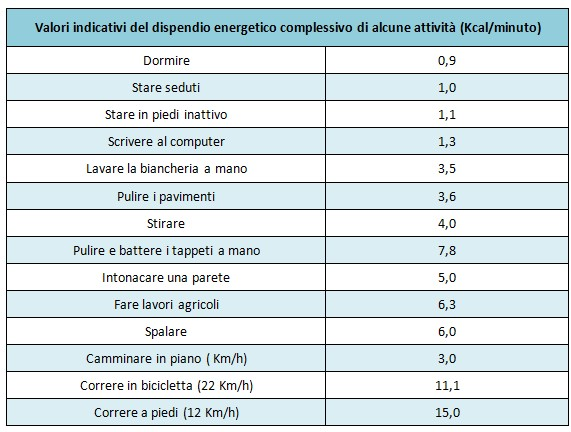
\includegraphics[width=0.7\textwidth]{20/image5.jpeg}
	\end{figure}

Come calcolare un adeguato apporto calorico?

LARN = Livelli di Assunzione di Riferimento di Nutrienti e di energia
(quarta revisione del 2014). Qui ci sono le indicazioni precise sul
fabbisogno calorico.

\begin{figure}[!ht]
\centering
	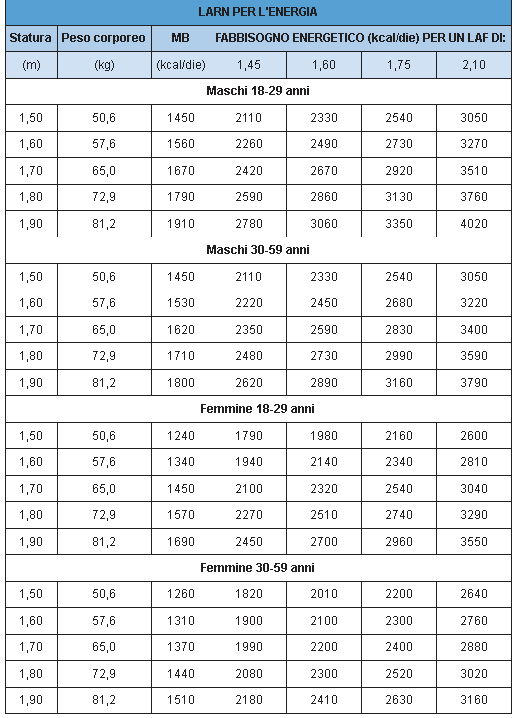
\includegraphics[width=0.7\textwidth]{20/image6.png}
	\end{figure}

Da questa tabella, ad esempio, possiamo capire quale sia il fabbisogno
energetico per i maschi e per le femmine dai 18-29 anni e dai 30-59
anni, in base all'altezza, al peso e all'attività svolta.

C'è una corrispondenza precisa tra statura e peso corporeo:

BMI (Body Mass Index)= peso (in kg)/altezza\textsuperscript{2} (in m)

L'evidenza scientifica ci dice che questo indice è l'indice che permette
di prevenire le patologie associate al sovrappeso: ad un determinato
indice si ritrova per entrambi i sessi la più bassa mortalità e quindi
la più bassa incidenza di patologie.

\begin{figure}[!ht]
\centering
	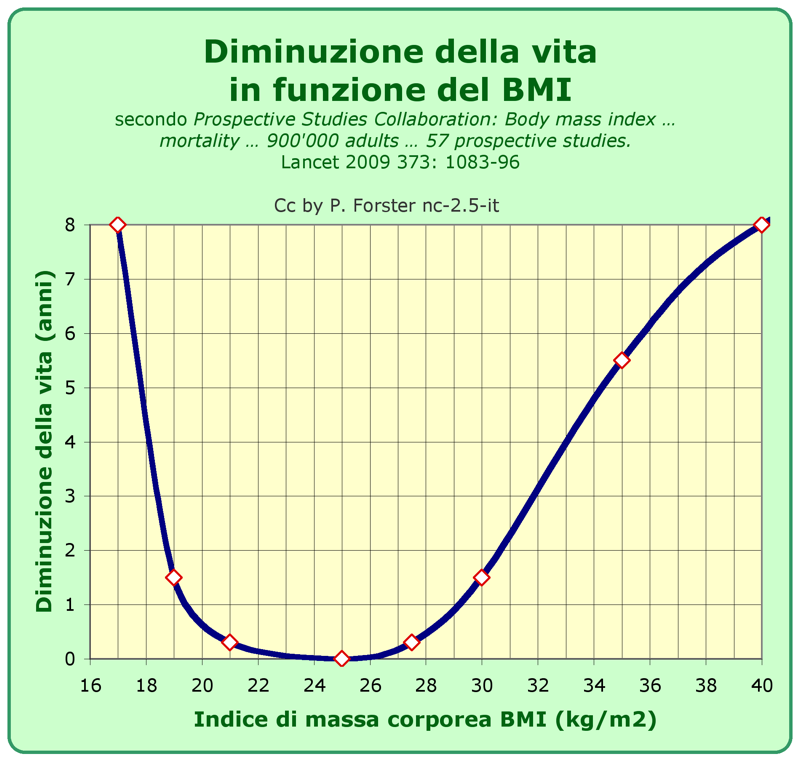
\includegraphics[width=0.7\textwidth]{20/image7.png}
	\end{figure}

Una dieta equilibrata deve fornire non solo un adeguato apporto
calorico, ma deve anche esserci un adeguato apporto di tutti i macro e
micro nutrienti perché svolgono diverse funzioni (ricorda l'importanza
delle vitamine lipo e idrosolubili e di fibre!). Quindi c'è indicazione
alla dieta mediterranea che comprende 25-30\% lipidi, glucidi 50\%,
protidi 12-15\% e fibre 25 grammi al giorno (sappiamo come siano
protettive per il tumore al colon-retto ).

È quindi necessario che la dieta sia varia e che un soggetto assuma
diversi alimenti a seconda dell'apporto che danno.

Sono quindi stati individuati 5 gruppi di alimenti:

\begin{itemize}
\item
  Funzionalità energetica dei cereali
\item
  Frutta e ortaggi per le vitamine e minerali (vario)
\item
  Latte e derivati per i lipidi, proteine e vit. liposolubili
\item
  Carne pesce, uova e legumi per proteine e grassi ( legumi + cereali =
  quota proteica di elevato valore biologico)
\item
  Grassi da condimento
\end{itemize}

\begin{figure}[!ht]
\centering
	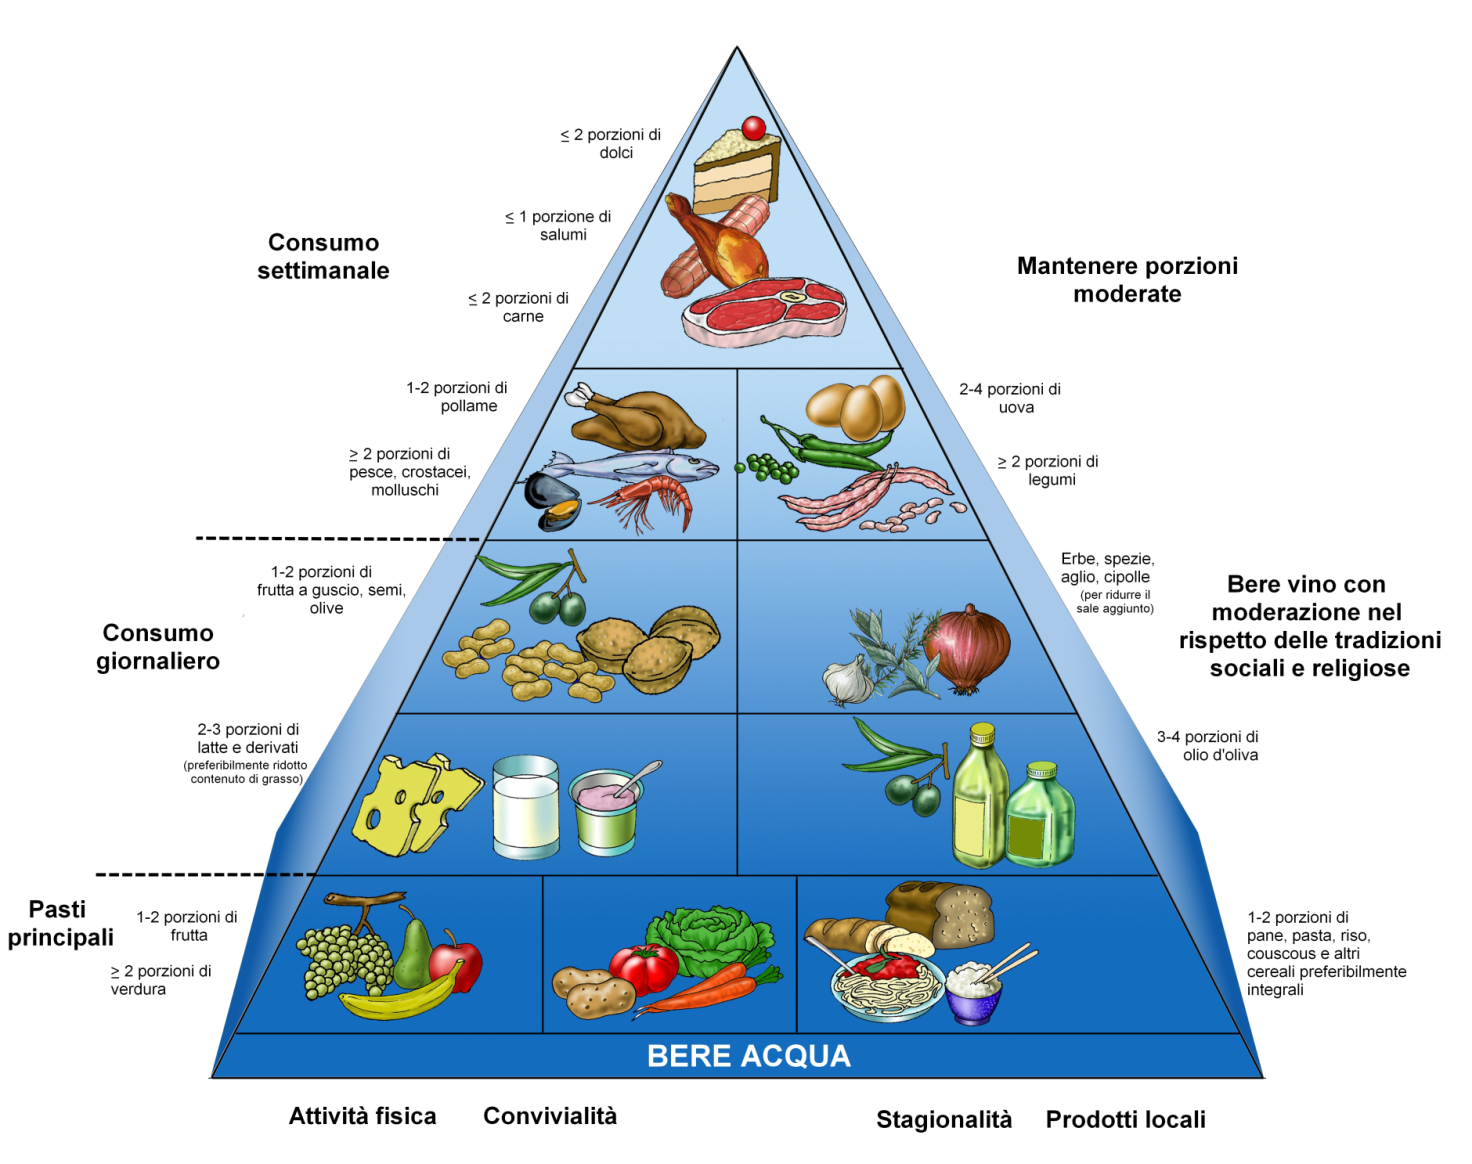
\includegraphics[width=0.7\textwidth]{20/image8.png}
	\end{figure}

Oltre all'apporto calorico totale e alla diversità dei nutrienti c'è un
altro aspetto importante: la cronologia dell'assunzione degli alimenti.
Essi devono essere distribuiti durante tutto il giorno, come sotto
riportato.

\begin{figure}[!ht]
\centering
	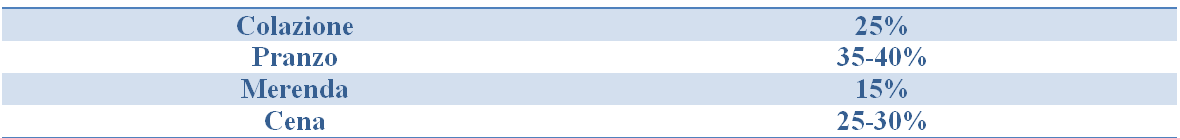
\includegraphics[width=0.7\textwidth]{20/image9.png}
	\end{figure}

Viene pertanto evidenziata l'importanza della colazione.

Già Ippocrate aveva individuato l'alimentazione come determinante di
salute.

Non c'è integratore alimentare che possa sostituire l'apporto degli
alimenti.

\subsection{Danni da alimentazione scorretta}

Quali possono essere i danni che derivano da un'alimentazione scorretta?

\begin{itemize}
\item
  Danni in eccesso
\item
  Danni in difetto
\end{itemize}

Questi danni possono riguardare tutte le componenti oppure solo una
componente specifica.

Nel mondo si ritrovano situazioni estreme: ogni anno muoiono milioni di
persone per mancanza di alimenti e milioni per eccesso di alimenti.

Nei paesi industrializzati i danni sono quasi sempre eccesso, anche se
si possono trovare carenze (per esempio il ferro nel periodo fertile
delle donne).

Quali sono i più frequenti errori alimentari?

\begin{itemize}
\item
  eccesso di introito generale, già cominciando da bambini;
\item
  eccesso in particolare di grassi, alimenti proteici , zuccheri
  semplici;
\item
  eccesso di sale;
\item
  eccesso di alcol;
\item
  carenza di fibre vegetali.
\end{itemize}

Nel grafico sottostante sono riportati dati del 1975; sull'asse delle
ordinate viene indicato il valore in percentuale del fabbisogno calorico
giornaliero. Già in quegli anni vi erano numerosi Paesi con apporto
calorico molto maggiore dei livelli raccomandati.

\begin{figure}[!ht]
\centering
	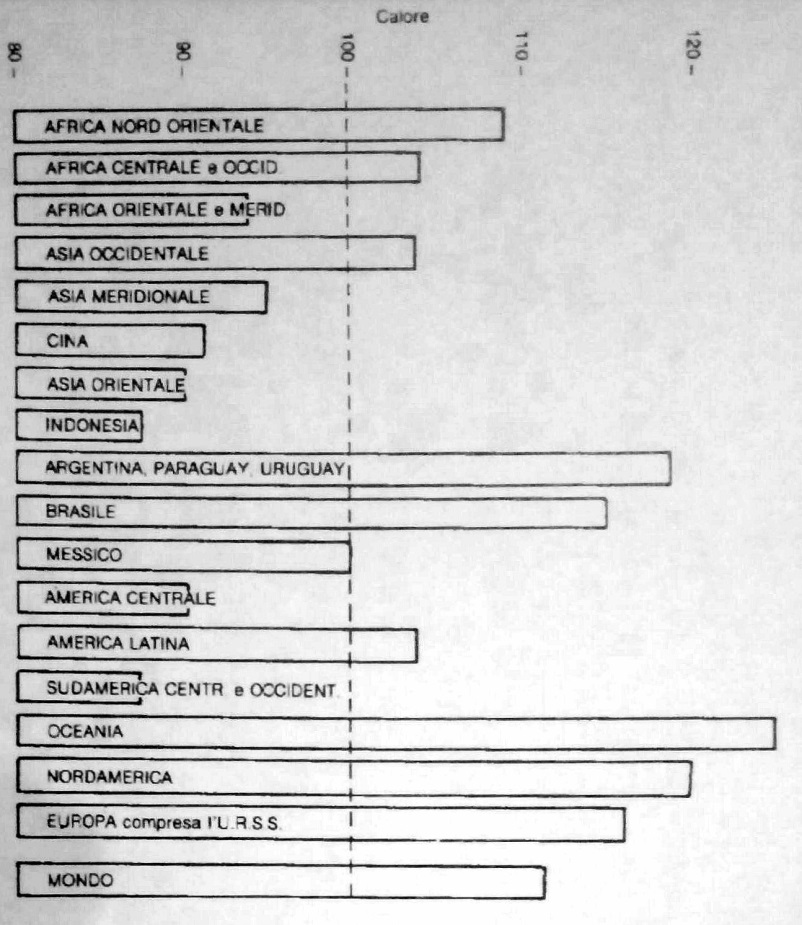
\includegraphics[width=0.7\textwidth]{20/image10.jpeg}
	\end{figure}

Dati registrati successivamente indicano un ulteriore aumento
dell'introito calorico; la quota che è aumentata è la \% di proteine e
grassi assunti (poiché è aumentato il consumo di carne e di grassi da
condimento) mentre si è ridotta (o comunque non è aumentata
proporzionalmente) la \% di carboidrati.

Altro punto critico è l'introito di sale; non bisognerebbe superare i 5
grammi al giorno.

In tutte le regioni si osserva una notevole differenza di assunzione
rispetto a quanto è raccomandato.

Importante è anche come tra i bambini manchi l'abitudine alla colazione
e avvenga invece una merenda abbondante, scarso apporto di frutta e
verdura ed eccesso di bevande gassate, il tutto associato ad una
mancanza di attività fisica.

\subsection{Patologie associate a scorretta alimentazione}

\begin{itemize}
\item
  Obesità
\item
  Patologie cardiovascolari (per esempio ipertensione legata al consumo
  di sale)
\item
  Diabete (eccesso di zuccheri)
\item
  Tumore colon (ridotto consumo di fibre, carenza di vitamine
  antiossidanti)
\end{itemize}

La scarsa assunzione di frutta e verdura è responsabile del 20\% dei
tumori GI e del 31\% delle cardiopatie ischemiche e ictus.

In un recente lavoro si vede anche l'associazione tra carenza di frutta
e verdura e morte per tumori al polmone o attacchi ischemici.

Il consumo fino a 600 grammi al giorno di frutta e verdura riduce la
mortalità fino al 2\% (mortalità per cardiopatia ischemica e ictus e per
tumori allo stomaco, esofago, polmoni, ecc.).

La prima conseguenza di una scorretta alimentazione con elevato apporto
di proteine e lipidi è il sovrappeso.

\subsubsection{Sovrappeso e obesità}

Oggi sovrappeso e obesità sono diventati un'epidemia a livello globale;
quello che preoccupa di più è che siano presenti nell'infanzia perché
bambini sovrappeso sono maggiormente predisposti a mantenere questa
situazione nel tempo. Inoltre nel bambino le cellule adipose sono in
grado di moltiplicarsi, mentre nell'adulto aumentano semplicemente di
volume: è quindi molto probabile che un bambino in sovrappeso diventi un
adulto in sovrappeso o obeso.

L'Italia detiene un triste primato a livello europeo: la prevalenza di
bambini tra 7 ed 11 anni in sovrappeso si attesta attorno al 36\%.

Negli adulti si può notare innanzitutto la diversità tra Nord e Sud,
regioni al di sotto della media e regioni al di sopra della media per
quanto riguarda l'eccesso ponderale e l'obesità. La \% di obesi e di
individui sovrappeso è maggiormente distribuita nelle regioni
meridionali.

Perché?

\begin{itemize}
\item
  Motivi culturali: si ritiene che il bambino cicciotto sia in buona
  salute.
\item
  Ridotta attività fisica: si utilizzano molto i mezzi per spostarsi a
  causa delle ridotte infrastrutture (per esempio piste ciclabili)
  oppure per la ridotta sicurezza nello spostarsi a piedi o in
  bicicletta.
\end{itemize}

Vi è anche un'associazione tra eccesso ponderale e istruzione e tra
eccesso ponderale e condizioni economiche (per es. frutta e verdura
costano di più, le merendine senza grassi idrogenati costano di più).

\begin{figure}[!ht]
\centering
	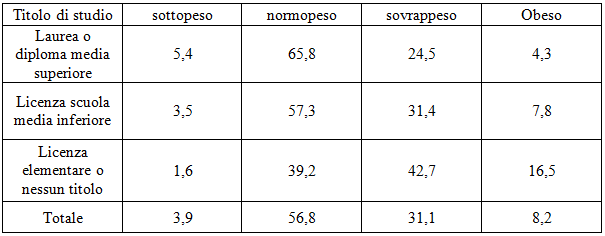
\includegraphics[width=0.7\textwidth]{20/image11.png}
	\end{figure}

Non basta essere consapevole di cosa fare per essere in salute ed
evitare i danni, ma posso trovarmi in situazioni dove non ho alimenti
sani a disposizione oppure non avere le possibilità economiche; è quindi
fondamentale che sia un approccio multisettoriale. Bisogna quindi
fornire i mezzi e le possibilità quali ad es. i parchi e tutte le
strutture necessarie, fornire una corretta istruzione e corrette
informazioni a riguardo. Bisogna quindi agire su determinanti sia
sanitari che non sanitari e lavorare sulle resistenze che si possono
incontrare.

Importante è anche lavorare sulla percezione del proprio peso: ci sono
persone che pur essendo obese non hanno la percezione della loro
situazione oggettiva. Il 10\% di obesi si vede giusto! Questo è un dato
che deve far riflettere. Quindi la consapevolezza risulta il primo step
fondamentale per poter cambiare.

Altro fattore importante è lo scarso interesse, anche dei medici di
medicina generale, riguardo questi aspetti del proprio paziente. Anche
dal punto di vista del servizio sanitario è fondamentale cambiare
atteggiamento.

Il problema è globale: GLOBESITY.

Molti Paesi superano il 50\% di soggetti sovrappeso, per es. l'Australia
rappresenta un picco. Le previsioni per il futuro non sono poi molto
favorevoli: in uno studio recente si vede come in diversi Paesi
l'obesità sarà in aumento.

Se non si cambierà la situazione ciò rappresenterà un costo enorme per
la spesa sanitaria.

Per esempio nel 60 \% delle morti premature per cause cardiovascolari si
è rilevato BMI\textgreater{}25; si evidenzia inoltre un'associazione tra
sovrappeso e patologie quali tumore della mammella, anche se non se ne
conosce il meccanismo alla base.

\subsubsection{Malattie cardiovascolari}

L'impatto è enorme in termini di morbosità per quanto riguarda la
cattiva alimentazione su questo tipo di patologie.

Di solito pensiamo subito alla Finlandia per quanto riguarda questo
argomento.

\begin{figure}[!ht]
\centering
	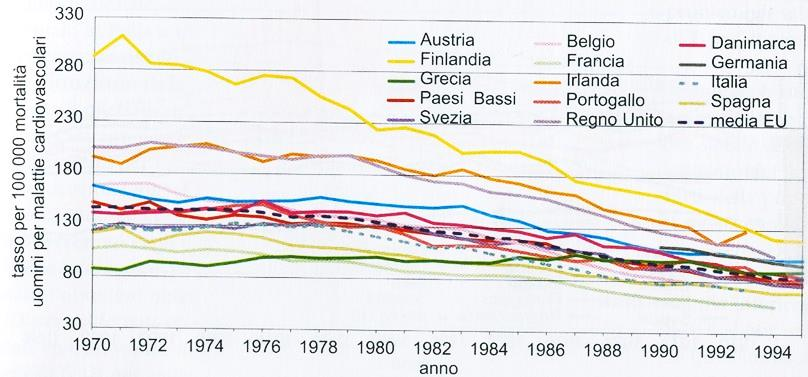
\includegraphics[width=0.7\textwidth]{20/image12.jpeg}
	\end{figure}

Dati epidemiologici mostrano che in Finlandia è molto al di sopra della
media europea. Qual è stato il problema? Questo paese è stato un modello
di studio per l'OMS di come le patologie cardiovascolari possano essere
prevenute.

In questo Paese è successo che la popolazione era costituita soprattutto
da boscaioli, la cui attività era di sollevare tronchi pesanti e quindi
l'introito calorico arrivava anche a 5000 kcal, estremamente elevato ma
in linea con l'attività fisica svolta. Quando sono arrivate le macchine
a sostituire la pesante attività fisica dell'uomo l'introito è rimasto
invariato, a fronte però di un'attività fisica molto ridotta. Allora è
cominciata questa incidenza elevatissima di accidenti cardiovascolari.

Qui si vede proprio il successo della prevenzione: una riduzione del
consumo calorico ha ridotto notevolmente l'incidenza di queste patologie
e della mortalità causata da queste.

Quindi riduzione del consumo di sale, perdita di peso, più consumo di
frutta e verdura sono le raccomandazioni da seguire.

Ricordiamo il ``Progetto Cuore'' dell'Istituto Superiore di Sanità,
definito come il primo passo per la prevenzione e la consapevolezza del
rischio. Qui viene stimato il rischio di sviluppare una patologia
cardiovascolare nel giro di 10 anni, in base ai seguenti fattori:

\begin{itemize}
\item
  Sesso
\item
  Diabete
\item
  Fumo
\item
  Età
\item
  Pressione sistolica
\item
  Colesterolemia
\end{itemize}

Alcuni sono associati ad un'alimentazione non corretta. In base a questi
dati la persona viene inserita in una delle sei categorie di rischio.

\subsubsection{Patologie oncologiche}

Per quanto riguarda i fattori di rischio delle patologie oncologiche
troviamo l'alimentazione, che è responsabile per il 30-35\%, e poi
troviamo l'alcol e l'obesità.

è stato addirittura calcolato il rischio attribuibile: quale percentuale
è stata attribuita all'alimentazione?

\begin{itemize}
\item
  Cancro del colon 70\%
\item
  Cancro prostata 75\%
\item
  Cancro mammella 50\%
\item
  Endometrio 50\%
\end{itemize}

È stato stimato anche il contributo di obesità ed alcol per patologie
oncologiche a carico di fegato, orofaringe, mammella, apparato digerente
e respiratorio superiore.

\paragraph{Alcol}

\begin{figure}[!ht]
\centering
	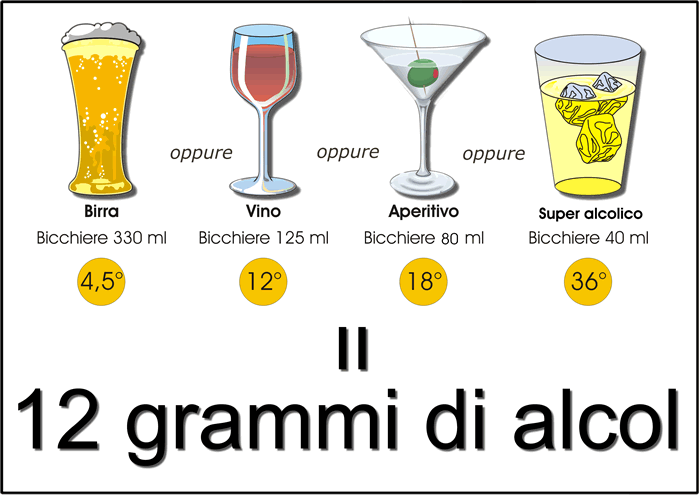
\includegraphics[width=0.7\textwidth]{20/image13.png}
	\end{figure}

1 unità alcolica = 12grammi di alcol = 1 boccale di birra = 1 bicchiere
di vino = 1 bicchierino di superalcolico = 7 kcal/g x 12g = 84kcal

Questa tabella mostra la riduzione dell' alcolemia nel tempo dopo
l'assunzione di alcol.

N.B. nel sesso femminile il metabolismo alcolico è più lento.

\begin{figure}[!ht]
\centering
	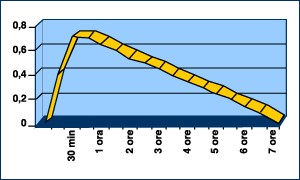
\includegraphics[width=0.7\textwidth]{20/image14.png}
	\end{figure}

Ricordiamo che il limite di legge è 0,50g/l per poter mettersi alla
guida.

Quali sono i danni correlati all'elevato consumo di alcol? Incidenti
stradali (già con un alcolemia al di sotto di 0,50 c'è riduzione della
visione laterale, peggioramento della coordinazione motoria quindi
un'alterazione della percezione e della reazione), tumori, infortuni,
cirrosi epatica, ecc\ldots{}

Oggi sono aumentati i bevitori \emph{binge:} soggetti che introducono
elevate quantità di alcol nello stesso momento (sono il 6\% dei
bevitori).

L'alcol permesso è al massimo 2 bicchieri di vino a giornata per il
sesso maschile e 1 per il sesso femminile.

\paragraph{Prevenzione}

Come sappiamo il primo passo è la sorveglianza, il monitoraggio, cioè
capire la situazione. In Italia è stata avviata la sorveglianza relativa
agli stili di vita quindi anche all'alimentazione e all'alcol per
soggetti \textgreater{}18 anni denominato SORVEGLIANZA P.A.S.S.I.
(Progressi delle Aziende Sanitarie per la Salute in Italia) proprio per
evocare questo miglioramento continuo che ci deve essere e che viene
monitorato.

Questi sono i temi che vengono indagati da questa sorveglianza:
alimentazione, attività fisica, alcol, fumo.

Poi abbiamo un altro sistema di sorveglianza nei bambini 8-9 anni; è un
monitoraggio continuo riguardo gli stili di vita.

Questi sistemi sono all'interno del progetto ``GUADAGNARE SALUTE''
dell'OMS, lanciato dal Ministero nel 2007. Questo progetto ha
l'obiettivo di intervenire sugli stili di vita in particolare
alimentazione, abuso di alcol, attività fisica e fumo.

Qual è lo slogan di questo progetto? \emph{Rendere facili le scelte
salutari} nella consapevolezza del nostro stile di vita che, secondo
l'OMS, è sì una nostra decisione, ma dipende anche dal contesto
socio-economico e culturale.

Quindi l'obiettivo è far sì che la scelta di salute sia più facilmente
accessibile per tutti gli ambiti.

Nell'ottica di quello che abbiamo detto non è sufficiente l'intervento
educativo, ma è necessario che contribuiscano tutti i settori nel
raggiungimento dell'obiettivo.

GUADAGNARE SALUTE è proprio un modello di promozione della salute,
apporto e sostegno di tutti i settori che hanno un ruolo nel migliorare
l'alimentazione, l'attività fisica, ecc.

Obiettivi:

\begin{itemize}
\item
  Promuovere i comportamenti salutari
\item
  Favorire l'alimentazione sana nella ristorazione
\item
  Informare i consumatori
\end{itemize}

Per ciascuno di questi obiettivi sono indicati gli attori: il Ministero
della salute, della pubblica istruzione, le aziende, l'ospedale, ecc.

Promozione di:

\begin{itemize}
\item
  Allattamento al seno
\item
  Sostenere la dieta mediterranea
\item
  Prevenire e monitorare i disturbi alimentari
\item
  Consumi salutari
\item
  Promuovere le risorse economiche
\item
  Informare i consumatori e tutelare i minori
\end{itemize}

Sono tutti compiti delle varie istituzioni; quindi gli interventi per
una corretta alimentazione hanno l'obiettivo di responsabilizzare
ciascuno di noi.

Un aspetto molto importante è anche la ristorazione collettiva visto che
oggi è molto diffuso consumare pasti al di fuori dell'ambiente
domestico.

Le linee guida quindi si trovano facilmente. Quali sono i punti
fondamentali?

\begin{itemize}
\item
  Più cereali, legumi, ortaggi e frutta
\item
  Limitare i grassi
\item
  Limitare il consumo di sale
\item
  Limitare gli zuccheri semplici
\item
  Limitare l'alcol e assumerlo in quantità molto controllata
\end{itemize}

Nell'ambito del progetto GUADAGNARE SALUTE vediamo per esempio
l'intervento per la riduzione del sale (per esempio riduzione del
consumo di pane ad alto contenuto di sale; ciò ha portato all'accordo
tra i panificatori per ridurre il contenuto di sale nel pane che è una
fonte elevata di sale).

Fondamentale anche l'intervento sull'età evolutiva, sono proprio stati
redatti dei documenti ad EXPO 2015 come le linee guida per la
comunicazione commerciale destinate ai bambini, documenti condivisi per
il miglioramento degli apporti nutritivi nei bambini.

Riguardo il riorientamento dei servizi sanitari per la promozione della
salute si auspica l'istituzione di servizi di \textbf{counceling
nutrizionale}, cioè il Servizio Sanitario Nazionale deve istituire dei
servizi che supportino i soggetti al cambiamento\textbf{.}

In questo piano si sottolinea l'importanza di agire poi nell'ambito
della scuola e dell'educazione dei bambini nella prima fascia di età. La
scuola è un ambito privilegiato perché i bambini sono in un'età in cui è
più facile fare proprie abitudini corrette, utilizzando gli insegnanti
come veicolo di informazione.
